\newif\ifimagen\imagentrue
\documentclass{article}
\usepackage{graphicx}
\usepackage{amsmath}
\usepackage{amsfonts}
\usepackage{amssymb}
\usepackage{stmaryrd}
\usepackage{makeidx}
\usepackage{times}
\usepackage{mathptmx}
\usepackage{ifpdf}
\usepackage[colorlinks,pdftex]{hyperref}
\usepackage[T1]{fontenc}
\newcommand{\R}{{\mathbb{R}}}
\newcommand{\C}{{\mathbb{C}}}
\newcommand{\Z}{{\mathbb{Z}}}
\newcommand{\N}{{\mathbb{N}}}
\newcommand{\faux}{$\square\;$}
\newcommand{\vrai}{$\boxtimes\;$}
\newcommand{\itemf}{\item\faux}
\newcommand{\itemvv}{\item\vrai}
\newcommand{\xcasin}[1]
{\begin{quote}\ttfamily
#1
\end{quote}}
\newcommand{\xcasout}[1]
{\begin{equation*}
#1
\end{equation*}}
\newtheorem{exo}{Exercise}[section]

\pagestyle{empty}
\thispagestyle{empty}
\begin{document}
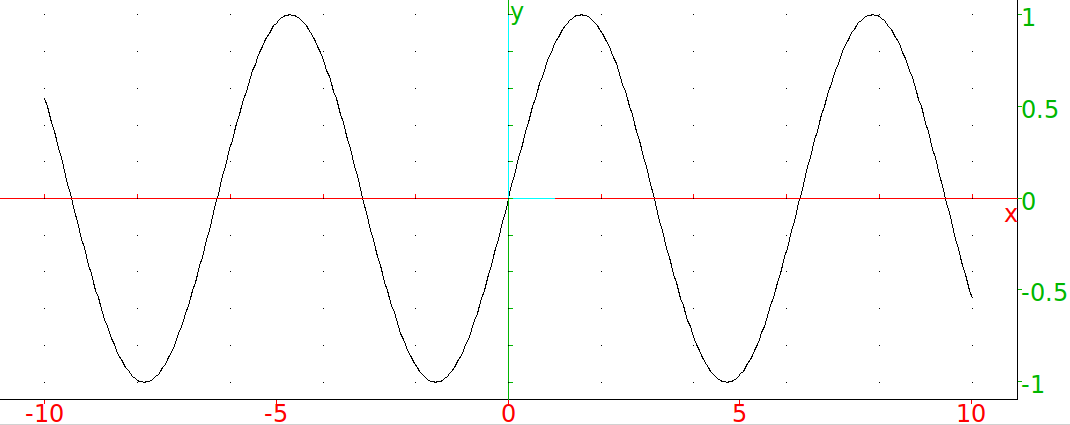
\includegraphics[width=\textwidth]{xcas-sinplot.png}
\clearpage% page: 0
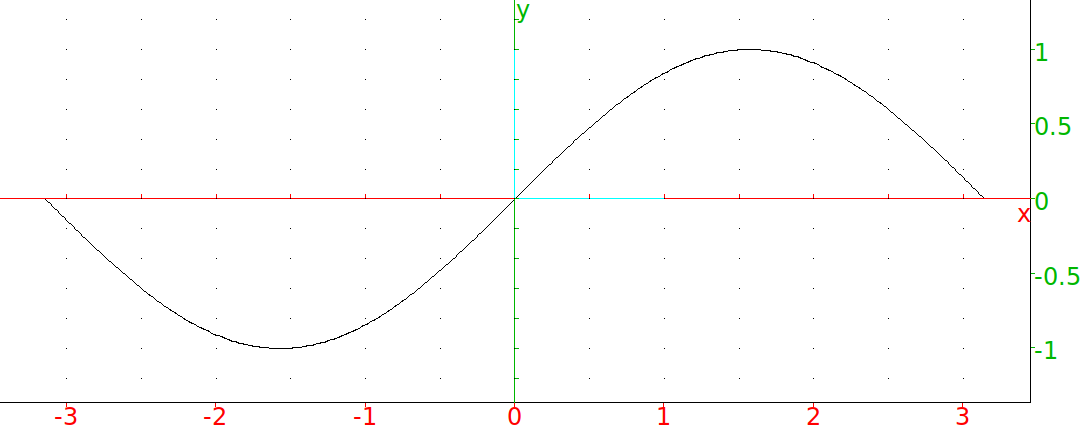
\includegraphics[width=\textwidth]{xcas-sinplot2.png}
\clearpage% page: 1
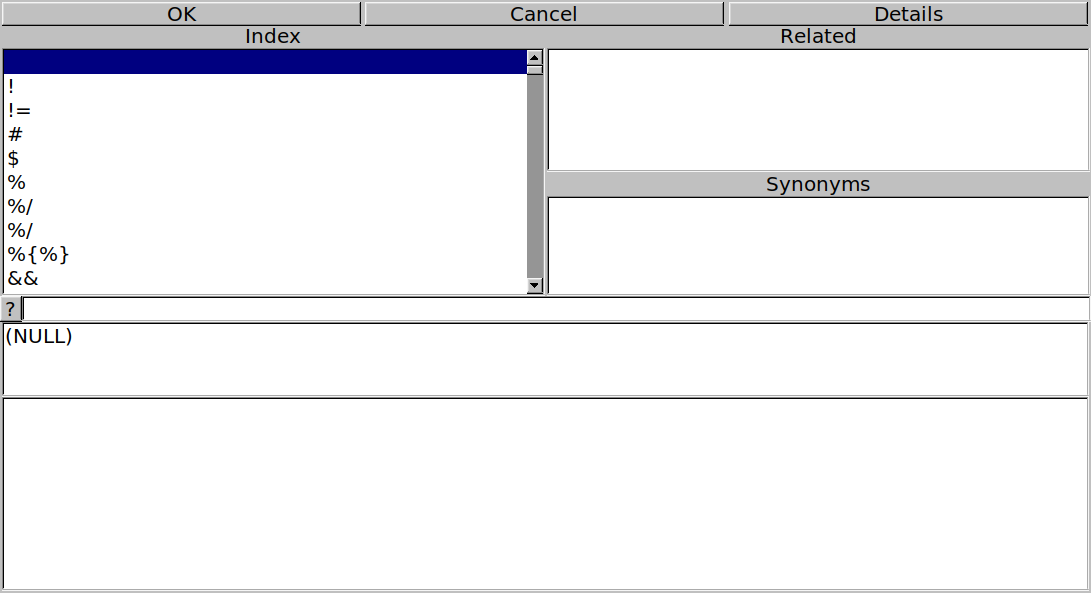
\includegraphics[width=\textwidth]{xcas-help-index.png}
\clearpage% page: 2
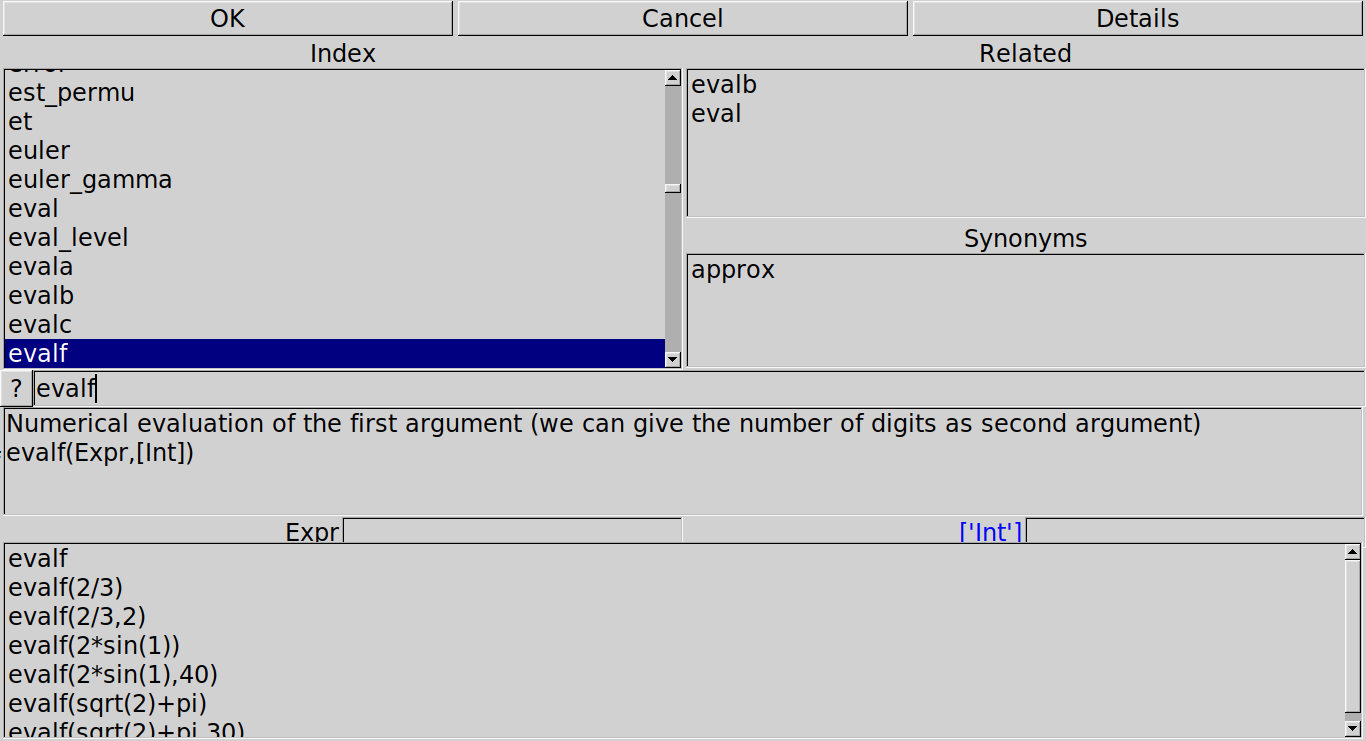
\includegraphics[width=\textwidth]{xcas-help-evalf.png}
\clearpage% page: 3
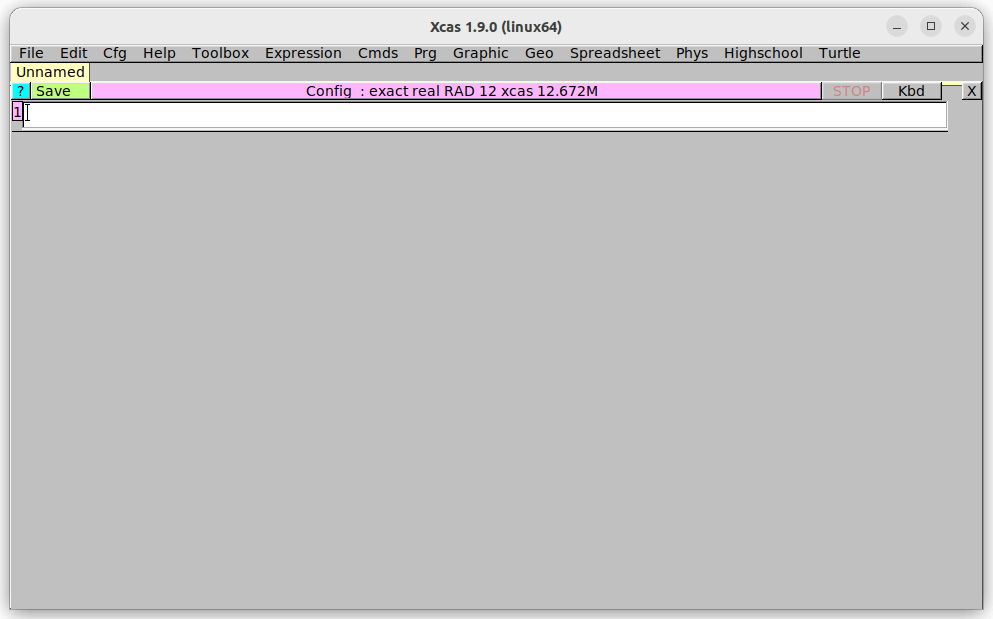
\includegraphics[width=\textwidth]{xcas-open.png}
\clearpage% page: 4
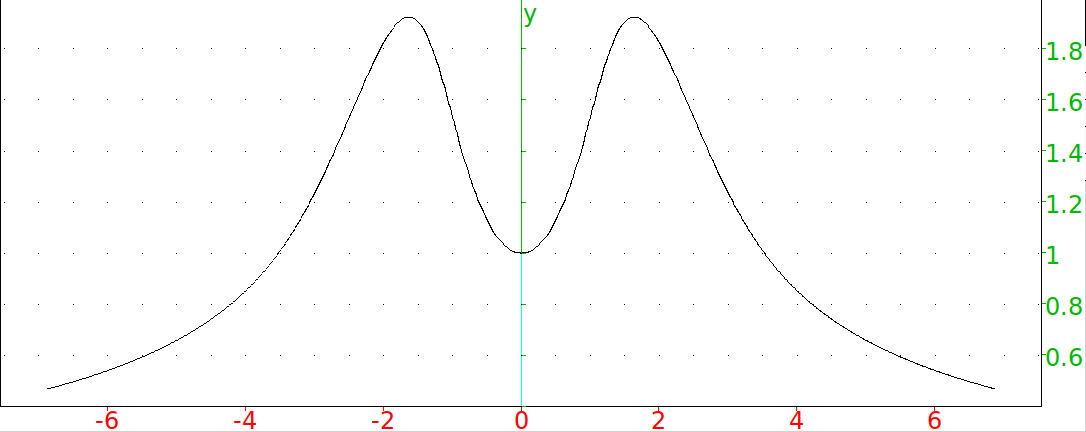
\includegraphics[width=\textwidth]{xcas-plotode.png}
\clearpage% page: 5
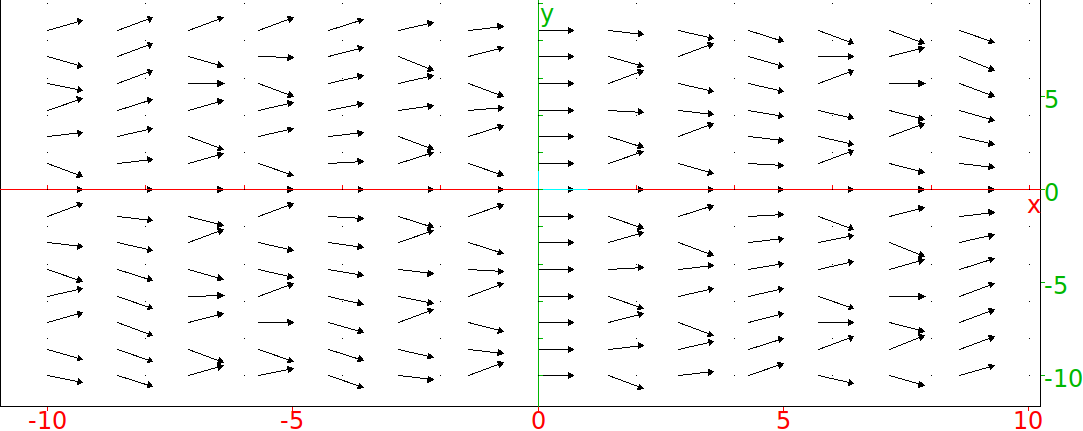
\includegraphics[width=\textwidth]{xcas-plotfield.png}
\clearpage% page: 6
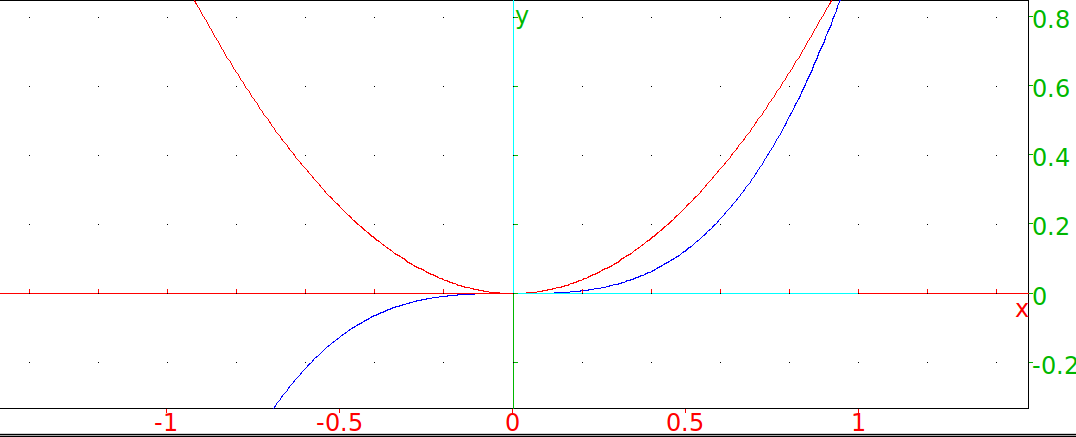
\includegraphics[width=\textwidth]{xcas-plot.png}
\clearpage% page: 7
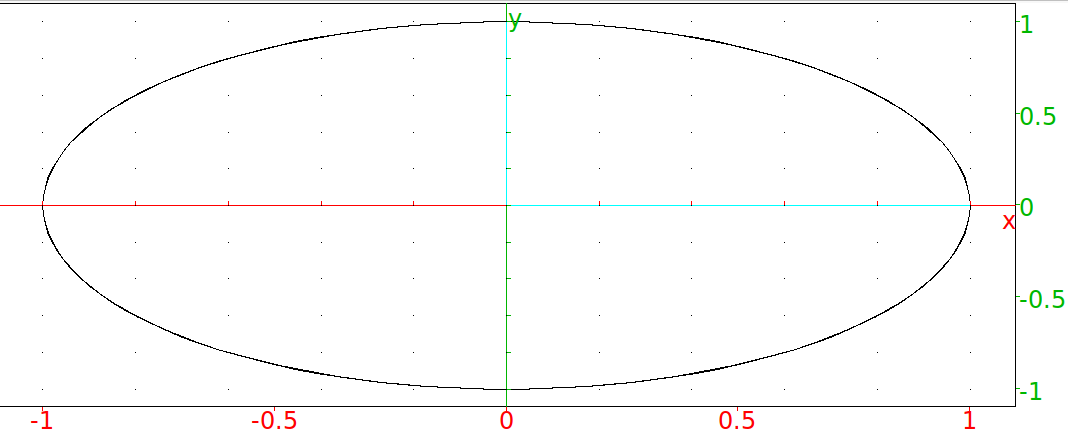
\includegraphics[width=\textwidth]{xcas-plotparam.png}
\clearpage% page: 8
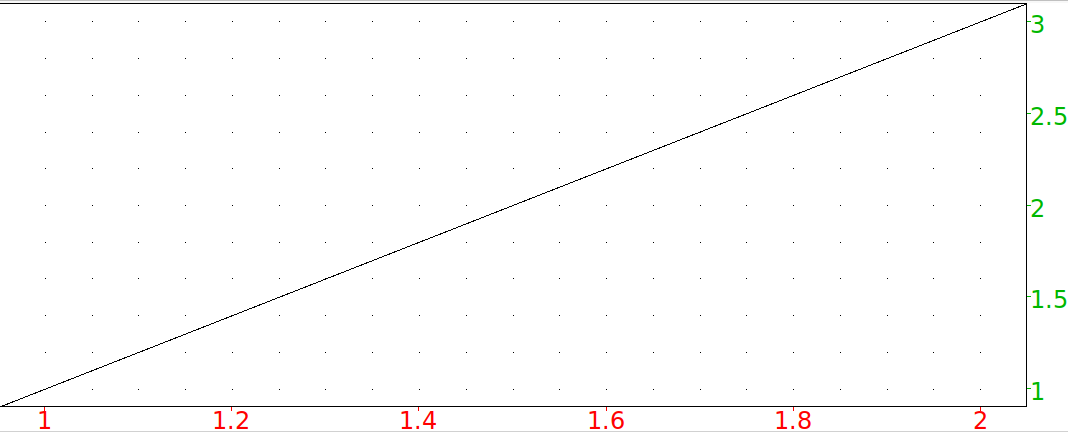
\includegraphics[width=\textwidth]{xcas-tangent.png}
\clearpage% page: 9
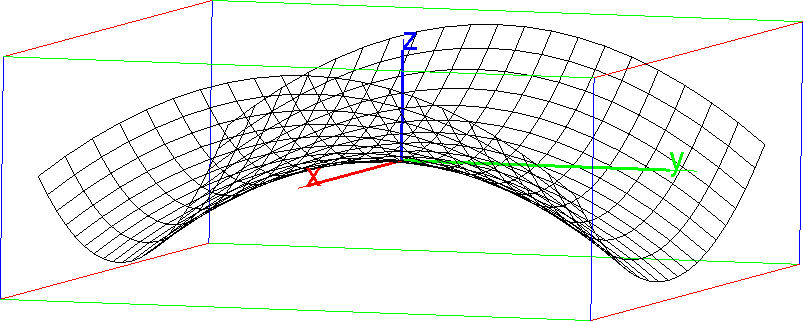
\includegraphics[width=\textwidth]{xcas-3dplot.png}
\clearpage% page: 10
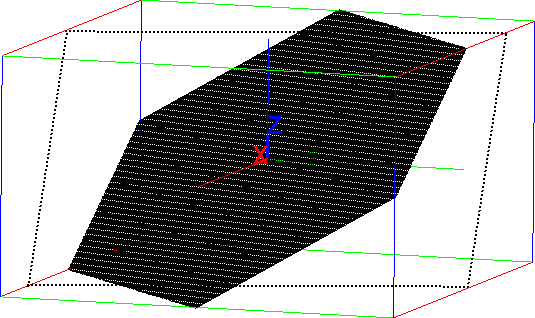
\includegraphics[width=\textwidth]{xcas-3dparam.png}
\clearpage% page: 11
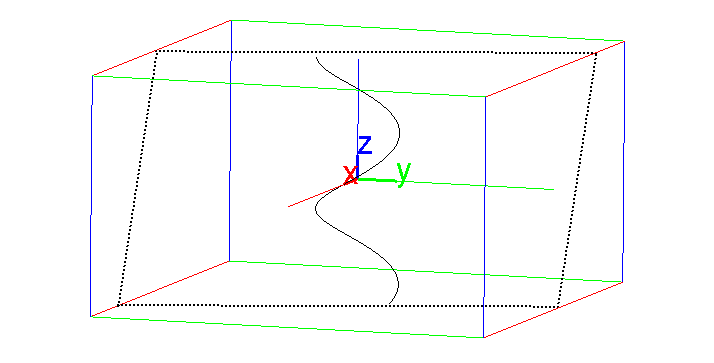
\includegraphics[width=\textwidth]{xcas-3dcurve.png}
\clearpage% page: 12
%Options: -png -pdf
\end{document}
